\documentclass{article}                                                   %
\usepackage{fullpage}                                                     %
\usepackage{pgffor}                                                       %
\usepackage{amssymb}                                                      %
\usepackage{Sweave}                                                       %
\usepackage{bm}                                                           %
\usepackage{mathtools}                                                    %
\usepackage{verbatim}                                                     %
\usepackage{appendix}                                                     %
\usepackage[UKenglish]{isodate} % for: \today                             %
\cleanlookdateon                % for: \today                             %
                                                                          %
\def\wl{\par \vspace{\baselineskip}}                                      %
\def\beginmyfig{\begin{figure}[htbp]\begin{center}}                       %
\def\endmyfig{\end{center}\end{figure}}                                   %
                                                                          %
\begin{document}                                                          %
% my title:                                                               %
\begin{center}                                                            %
  \section*{\textbf{Stat536 Midterm - Ozone Data}}                        %
  \subsection*{\textbf{Arthur Lui}}                                       %
  \subsection*{\noindent\today}                                           %
\end{center}                                                              %
\setkeys{Gin}{width=1\textwidth}                                          %
%%%%%%%%%%%%%%%%%%%%%%%%%%%%%%%%%%%%%%%%%%%%%%%%%%%%%%%%%%%%%%%%%%%%%%%%%%%

\section{Introduction: Problem Statement \& Goals}

    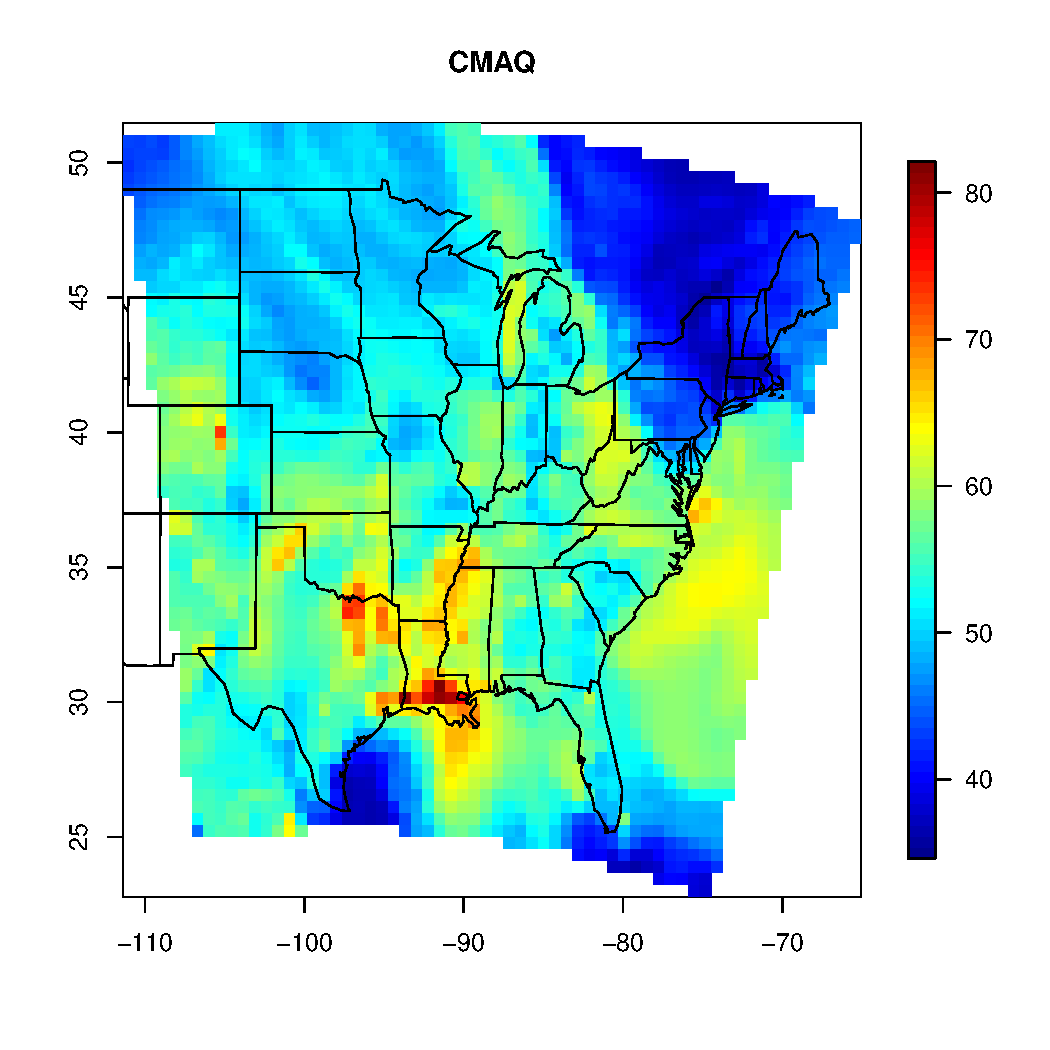
\includegraphics{raw/cmaq.pdf}
    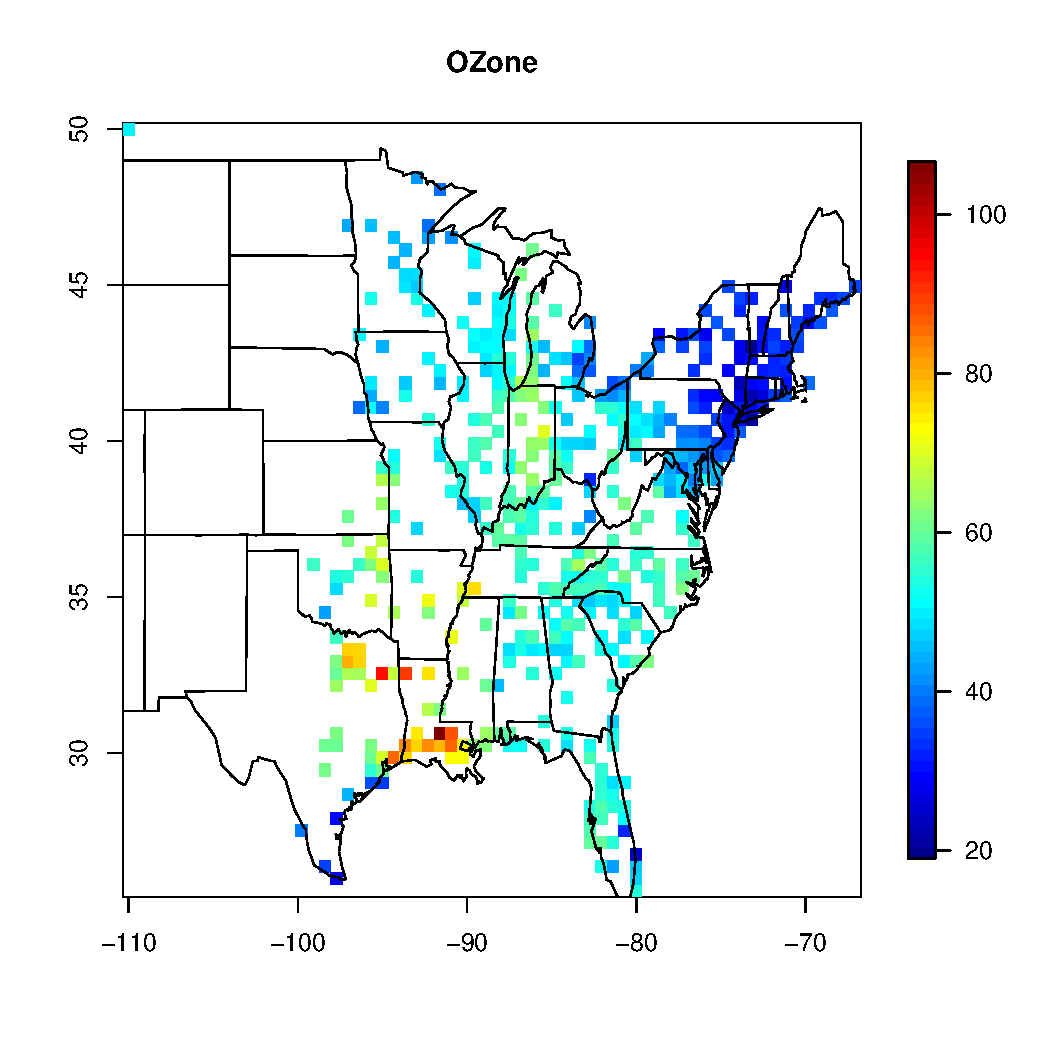
\includegraphics{raw/ozone.pdf}

\section{Method \& Model}
  \subsection{Brief Description of method / models used}
  \subsection{Assumptions}
\section{Model Justification}
  \subsection{Why choose a Gaussian Process?}
  \subsection{How does the GP solve the problem?}
  \subsection{Are Assumptions Justified?}
    \includegraphics{raw/resids.pdf}
    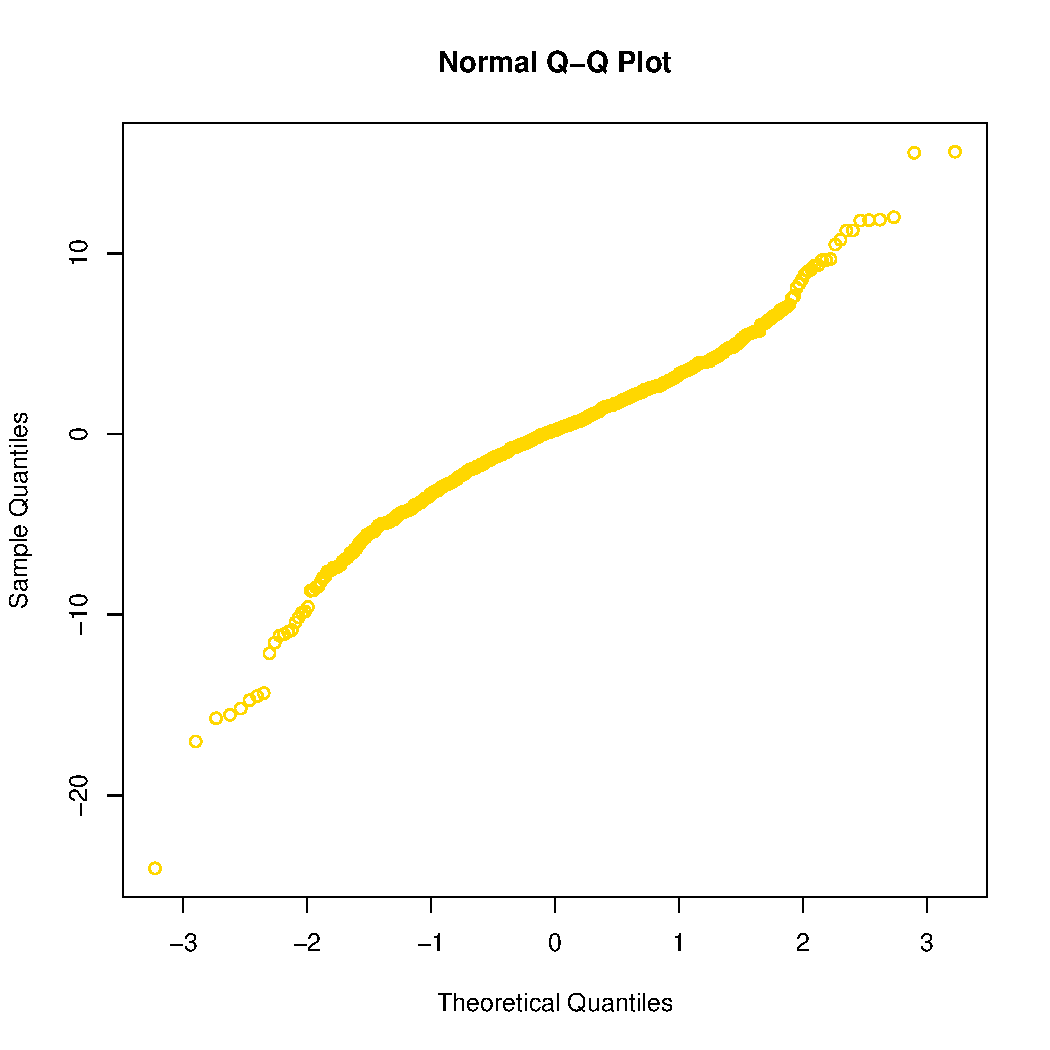
\includegraphics{raw/qqnorm.pdf}
    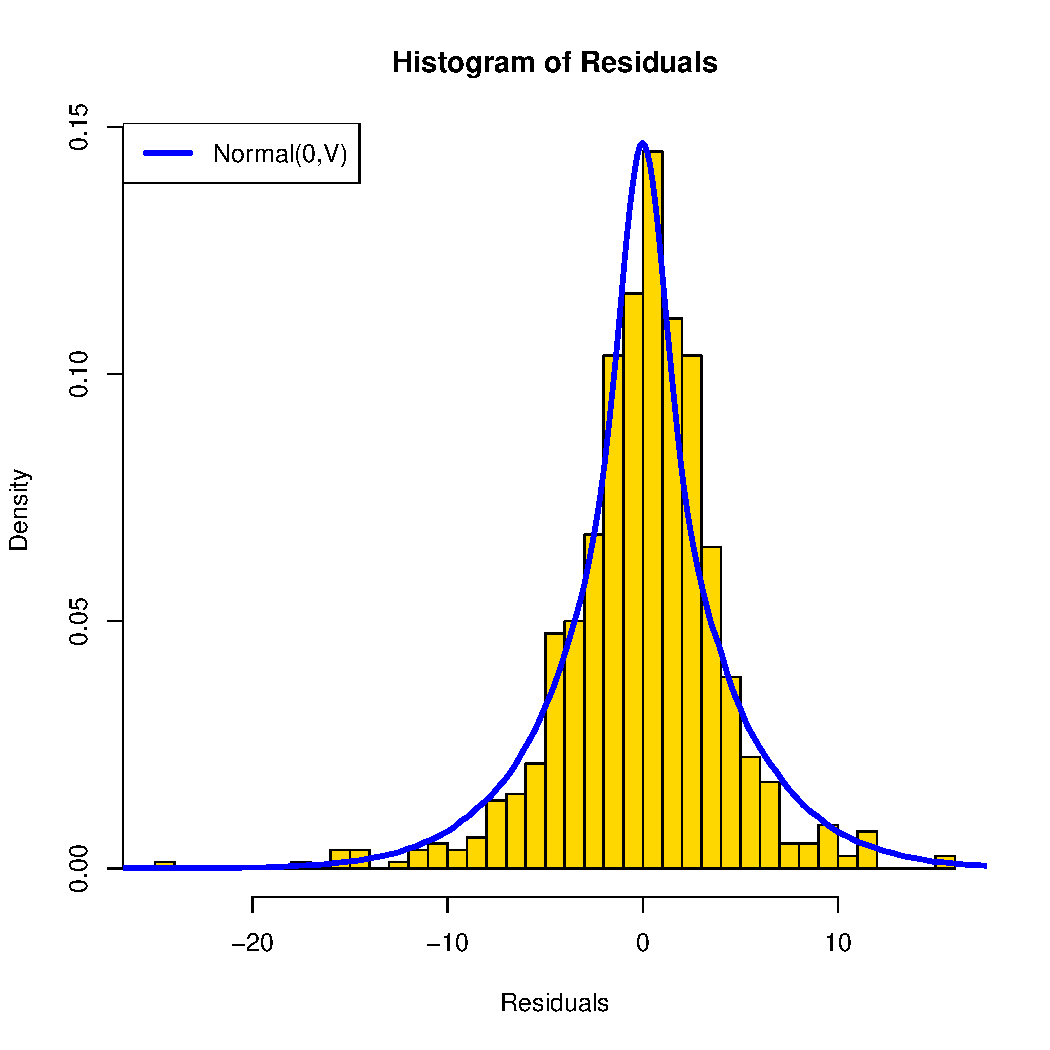
\includegraphics{raw/hist.pdf}
\section{Results}
  \subsection{Estimates of Parameters and CI}
    % latex table generated in R 3.0.2 by xtable 1.7-1 package
% Tue Mar  4 16:51:56 2014
\begin{table}[ht]
\centering
\begin{tabular}{rrrr}
  \hline
 & Estimates & CI.Lo & CI.Hi \\ 
  \hline
beta0 & 7.93766 & 1.29157 & 14.58375 \\ 
  beta1 & -0.11039 & -0.26032 & 0.03954 \\ 
  beta2 & 0.20544 & 0.06538 & 0.34549 \\ 
  beta3 & 0.08400 & -0.04960 & 0.21761 \\ 
  beta4 & 0.20130 & 0.06727 & 0.33534 \\ 
  beta5 & -0.11577 & -0.24077 & 0.00924 \\ 
  beta6 & 0.17512 & 0.05527 & 0.29497 \\ 
  beta7 & 0.14480 & 0.01922 & 0.27037 \\ 
  beta8 & 0.09521 & -0.01989 & 0.21031 \\ 
  beta9 & 0.06374 & -0.06132 & 0.18880 \\ 
  beta10 & 0.04647 & -0.06892 & 0.16187 \\ 
   \hline
\end{tabular}
\end{table}

    \[
      \begin{pmatrix}
        \hat{\tau^2} \\
        \hat{\sigma^2} \\
        \hat{\phi}
      \end{pmatrix} =
      \begin{pmatrix} 19.61\\1.04\\40.99 \end{pmatrix}
    \]
  \subsection{Coverage \& MSE }
    % latex table generated in R 3.0.2 by xtable 1.7-1 package
% Tue Mar  4 16:35:59 2014
\begin{table}[ht]
\centering
\begin{tabular}{rrrr}
  \hline
 & Estimate & CI.Lower & CI.Upper \\ 
  \hline
Coverage & 0.931 & 0.913 & 0.949 \\ 
  MSE & 20979.047 & 11019.079 & 30939.014 \\ 
   \hline
\end{tabular}
\end{table}

  \subsection{Predictions \& Uncertainties}
    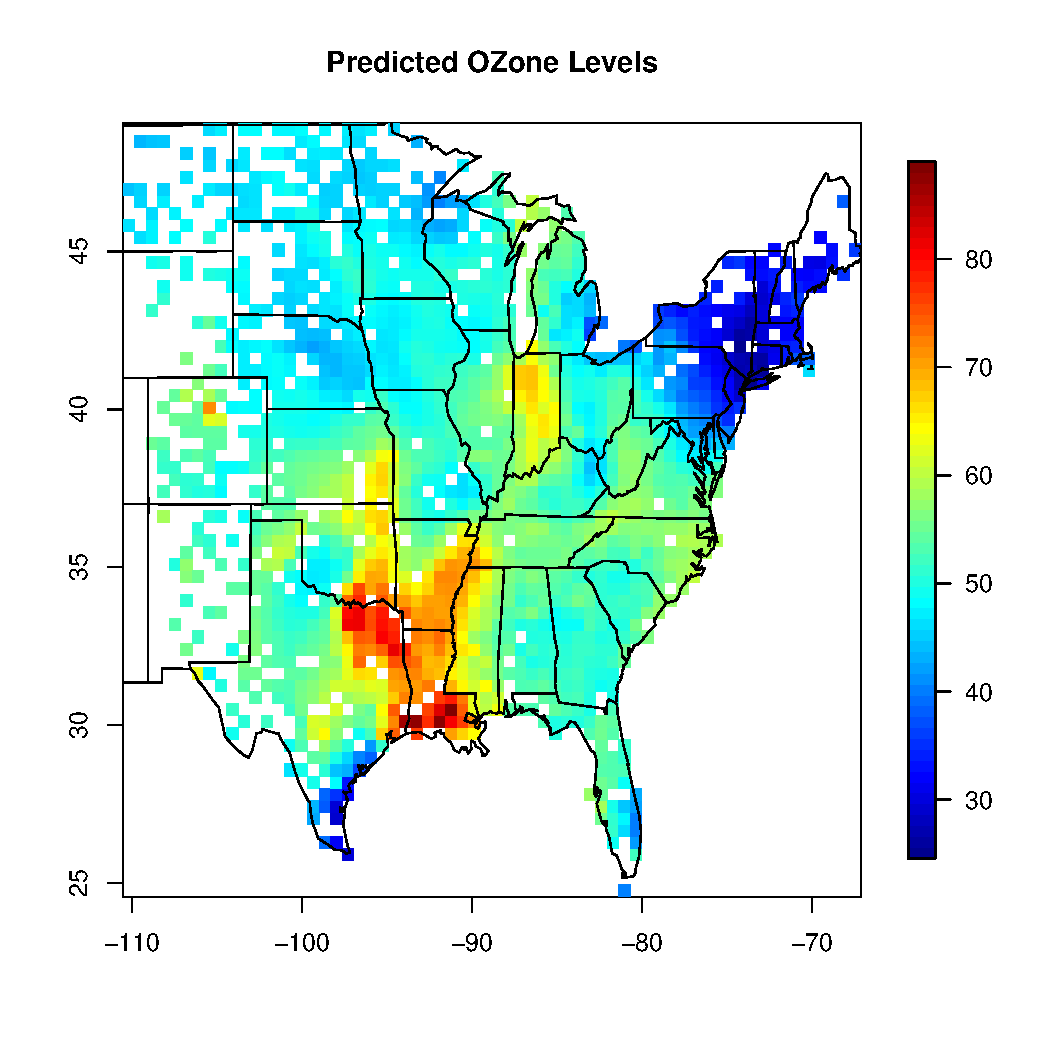
\includegraphics{raw/center.pdf}
    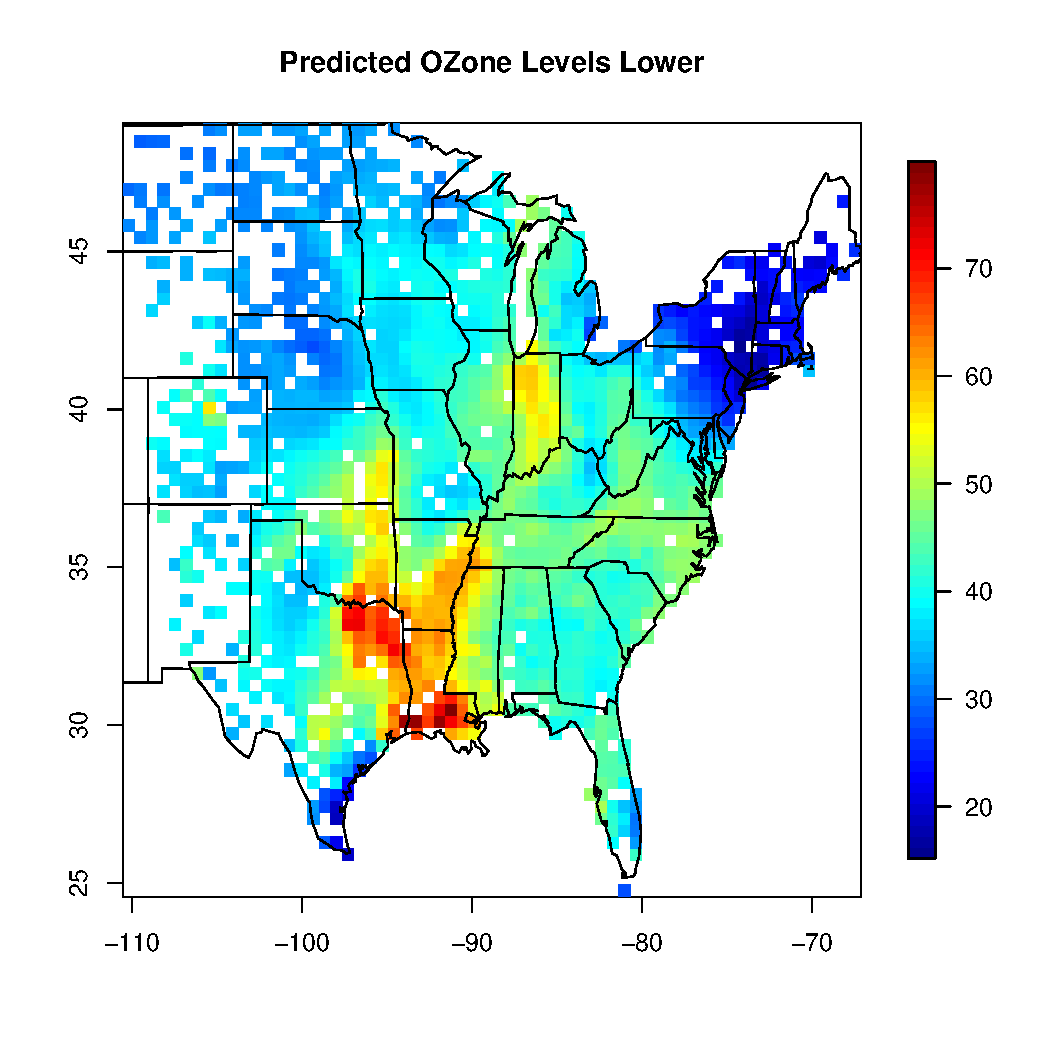
\includegraphics{raw/lower.pdf}
    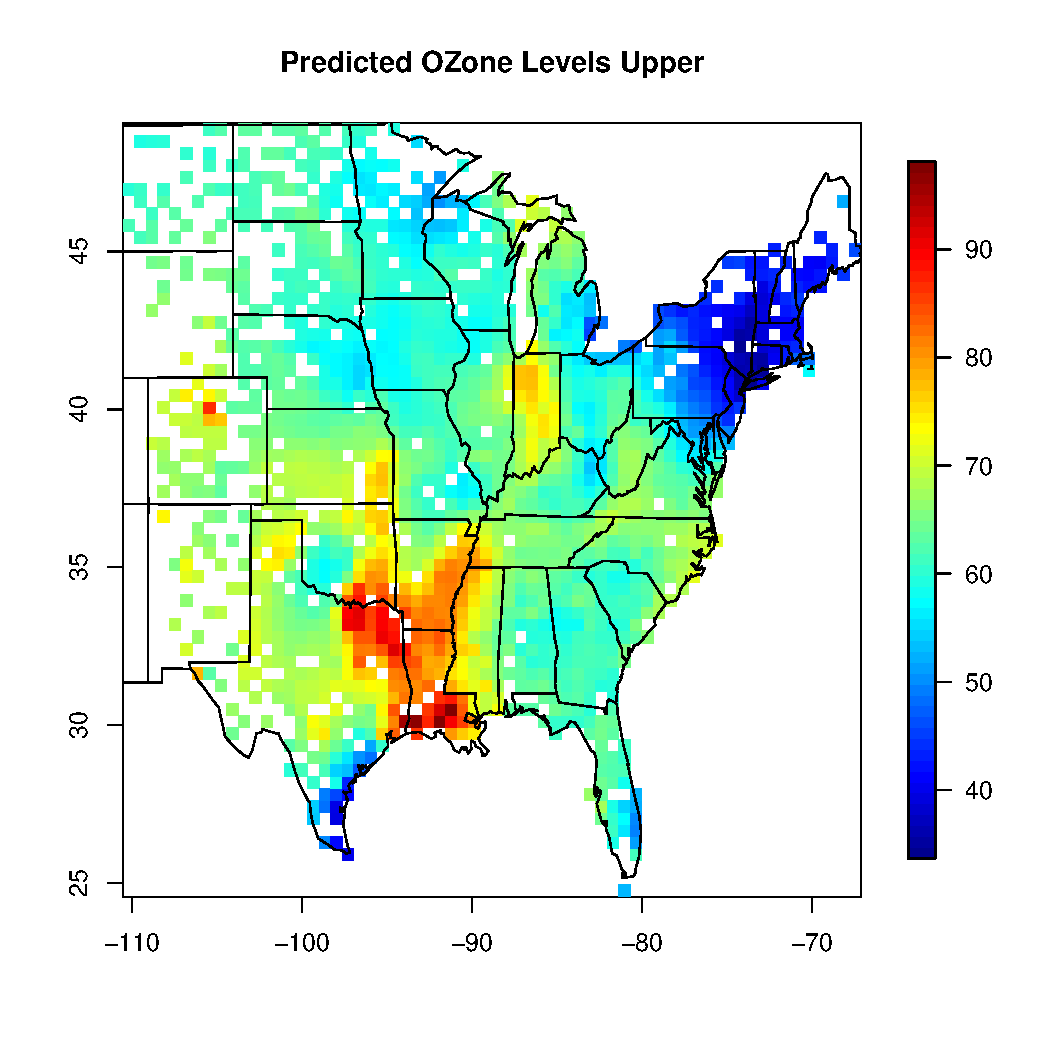
\includegraphics{raw/upper.pdf}
  \subsection{Interpretation}
  \subsection{Summary of Main Points}
    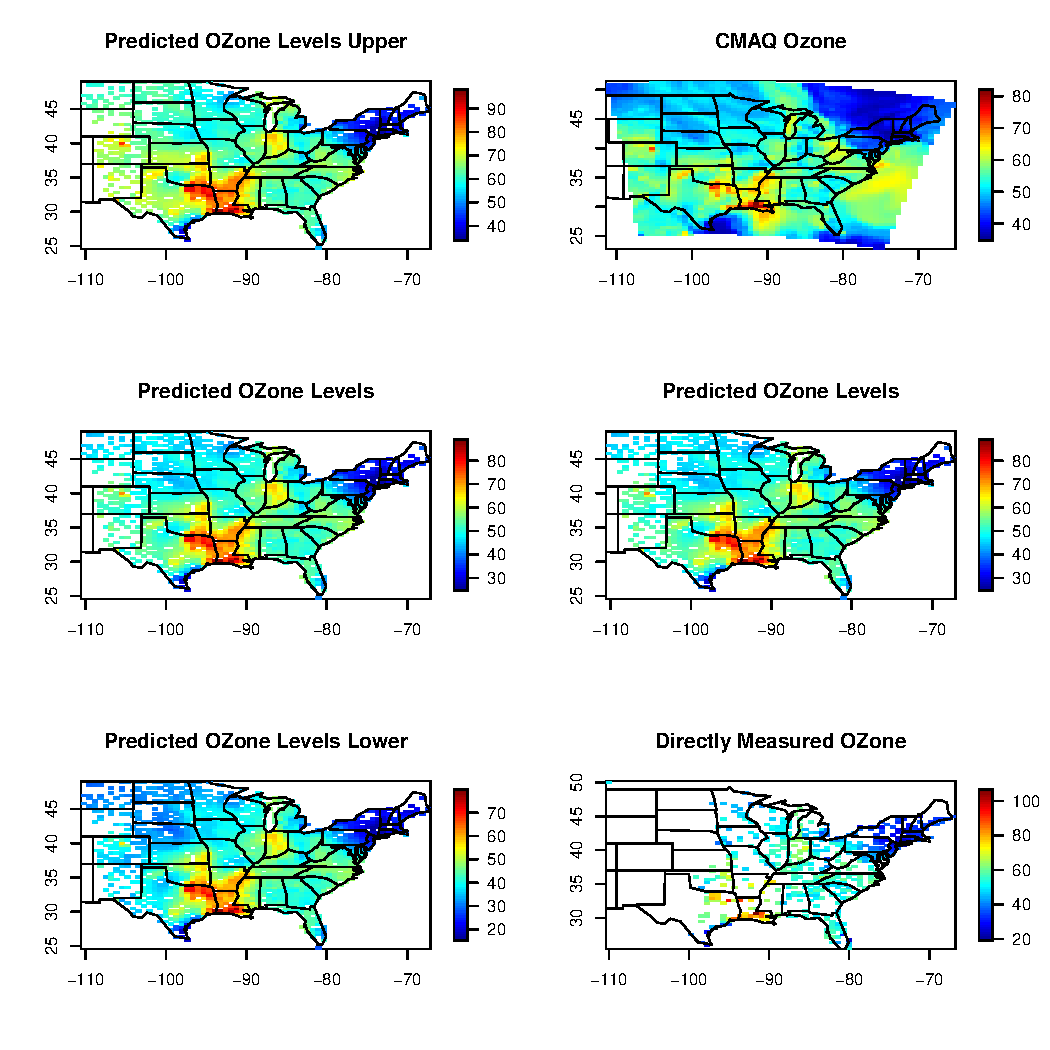
\includegraphics{raw/all.pdf}
\section{Conclusion}
  \subsection{Potential Alternative Approaches}
  \subsection{Shortcomings of GP or the way covars were chosen}
  \subsection{Further Investigation}
\end{document}
